\documentclass{standalone}
\usepackage{hsbcommon}
\usepackage{pgfplots}
\pgfplotsset{compat=1.18}
\begin{document}
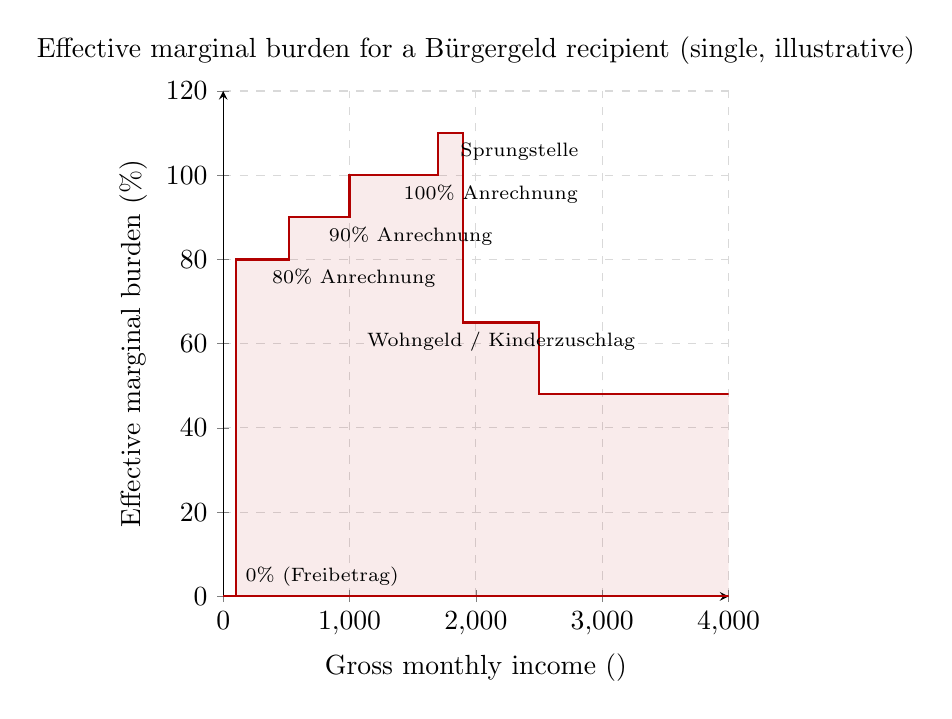
\begin{tikzpicture}
\begin{axis}[
    width=8cm, height=8cm,
    xlabel={Gross monthly income (\euro{})},
    ylabel={Effective marginal burden (\%)},
    xmin=0, xmax=4000,
    ymin=0, ymax=120,
    xtick={0,1000,2000,3000,4000,5000,6000},
    ytick={0,20,40,60,80,100,120},
    grid=major,
    grid style={dashed, gray!30},
    axis lines=left,
    title={Effective marginal burden for a Bürgergeld recipient (single, illustrative)},
]

\addplot[thick, color=red!70!black, mark=none, fill=red!70!black, fill opacity=0.08] coordinates {
    (0,    0)
    (100,  0)
    (100, 80)
    (520, 80)
    (520, 90)
    (1000, 90)
    (1000,100)
    (1700,100)
    (1700,110)
    (1900,110)
    (1900, 65)
    (2500, 65)
    (2500, 48)
    (6000, 48)
} \closedcycle;

\node[above right, font=\scriptsize] at (axis cs:100,0) {0\% (Freibetrag)};
\node[below right, font=\scriptsize] at (axis cs:310,80) {80\% Anrechnung};
\node[below right, font=\scriptsize] at (axis cs:760,90) {90\% Anrechnung};
\node[below right, font=\scriptsize] at (axis cs:1350,100) {100\% Anrechnung};
\node[below right, font=\scriptsize] at (axis cs:1800,110) {Sprungstelle};
\node[below, font=\scriptsize] at (axis cs:2200,65) {Wohngeld / Kinderzuschlag};
\node[below right, font=\scriptsize] at (axis cs:4500,48) {regulärer Steuer-/SV-Grenzsatz};

\end{axis}
% \node[font=\scriptsize, align=left, text width=13cm] at (3.5,-1.2) {
%     Hinweis: Stilisierte, illustrative Darstellung für einen alleinstehenden, kinderlosen Bürgergeld-Haushalt.
%     Der tatsächliche Verlauf hängt stark vom Haushaltstyp (Kinder, Miethöhe für Wohngeld, Kita-Gebührenstaffel etc.) ab.
% };
\end{tikzpicture}
\end{document}